% Robert Adams CS 475

\documentclass[letterpaper,10pt]{article} %twocolumn titlepage 
\usepackage{graphicx}
\usepackage{amssymb}
\usepackage{amsmath}
\usepackage{amsthm}

\usepackage{alltt}
\usepackage{float}
\usepackage{color}
\usepackage{url}

\usepackage{balance}
\usepackage[TABBOTCAP, tight]{subfigure}
\usepackage{enumitem}
\usepackage{pstricks, pst-node}


\usepackage{geometry}
\geometry{margin=1in, textheight=8.5in} %textwidth=6in

%random comment

\newcommand{\cred}[1]{{\color{red}#1}}
\newcommand{\cblue}[1]{{\color{blue}#1}}

\usepackage{hyperref}

\def\name{Robert Adams}
%% The following metadata will show up in the PDF properties
\hypersetup{
    colorlinks = true,
    urlcolor = black,
    pdfauthor = {\name},
    pdfkeywords = {cs745},
    pdftitle = {CS 475 Project 5: OpenMP: N-body Problem},
    pdfsubject = {CS 475 Project 5},
    pdfpagemode = UseNone,
}


\begin{document}
\title{CS 475 Project 5: OpenMP: N-body Problem}
\author{Robert Adams}
\maketitle



\section{Results}

The drop at around 8 threads is definitely of interest here.
This pattern seems to follow the class example of a program with cache misses.
 This seems to be an issue with the for loop on line 114. With these
 lines commented out the program shows more expected results without any dips. 


I would guess that the abysmal performance on the fine threading
above 2 threads may be because the overhead of constantly creating 
and joining threads exceeds the benefit of the time savings which they 
are able to give. There seems to be a sweet point for the amount of
work each thread should be given to maximize performance. 


The directive for the course threading placed above the for loop with int i looks as follows:

\verb|#|pragma omp parallel for default(none) private(Bodies) schedule(dynamic) 

The directive for the fine threading looks like:

\verb|#|pragma omp parallel for default(none) private(Bodies) shared(bi) reduction(+:fx, fy, fz) schedule(static)


\subsection{System Specifications}

access.engr.oregonstate.edu   lscpu:

Architecture:          x86\verb|_|64

CPU op-mode(s):        32-bit, 64-bit

Byte Order:            Little Endian

CPU(s):                8

On-line CPU(s) list:   0-7

Thread(s) per core:    1

Core(s) per socket:    4

CPU socket(s):         2

NUMA node(s):          1

Vendor ID:             GenuineIntel

CPU family:            6

Model:                 23

Stepping:              6

CPU MHz:               3166.000

BogoMIPS:              6317.53

Virtualization:        VT-x

L1d cache:             32K

L1i cache:             32K

L2 cache:              6144K

NUMA node0 CPU(s):     0-7


\begin{figure} [ht]
    \centering
    % GNUPLOT: LaTeX picture with Postscript
\begingroup
  \makeatletter
  \providecommand\color[2][]{%
    \GenericError{(gnuplot) \space\space\space\@spaces}{%
      Package color not loaded in conjunction with
      terminal option `colourtext'%
    }{See the gnuplot documentation for explanation.%
    }{Either use 'blacktext' in gnuplot or load the package
      color.sty in LaTeX.}%
    \renewcommand\color[2][]{}%
  }%
  \providecommand\includegraphics[2][]{%
    \GenericError{(gnuplot) \space\space\space\@spaces}{%
      Package graphicx or graphics not loaded%
    }{See the gnuplot documentation for explanation.%
    }{The gnuplot epslatex terminal needs graphicx.sty or graphics.sty.}%
    \renewcommand\includegraphics[2][]{}%
  }%
  \providecommand\rotatebox[2]{#2}%
  \@ifundefined{ifGPcolor}{%
    \newif\ifGPcolor
    \GPcolorfalse
  }{}%
  \@ifundefined{ifGPblacktext}{%
    \newif\ifGPblacktext
    \GPblacktexttrue
  }{}%
  % define a \g@addto@macro without @ in the name:
  \let\gplgaddtomacro\g@addto@macro
  % define empty templates for all commands taking text:
  \gdef\gplbacktext{}%
  \gdef\gplfronttext{}%
  \makeatother
  \ifGPblacktext
    % no textcolor at all
    \def\colorrgb#1{}%
    \def\colorgray#1{}%
  \else
    % gray or color?
    \ifGPcolor
      \def\colorrgb#1{\color[rgb]{#1}}%
      \def\colorgray#1{\color[gray]{#1}}%
      \expandafter\def\csname LTw\endcsname{\color{white}}%
      \expandafter\def\csname LTb\endcsname{\color{black}}%
      \expandafter\def\csname LTa\endcsname{\color{black}}%
      \expandafter\def\csname LT0\endcsname{\color[rgb]{1,0,0}}%
      \expandafter\def\csname LT1\endcsname{\color[rgb]{0,1,0}}%
      \expandafter\def\csname LT2\endcsname{\color[rgb]{0,0,1}}%
      \expandafter\def\csname LT3\endcsname{\color[rgb]{1,0,1}}%
      \expandafter\def\csname LT4\endcsname{\color[rgb]{0,1,1}}%
      \expandafter\def\csname LT5\endcsname{\color[rgb]{1,1,0}}%
      \expandafter\def\csname LT6\endcsname{\color[rgb]{0,0,0}}%
      \expandafter\def\csname LT7\endcsname{\color[rgb]{1,0.3,0}}%
      \expandafter\def\csname LT8\endcsname{\color[rgb]{0.5,0.5,0.5}}%
    \else
      % gray
      \def\colorrgb#1{\color{black}}%
      \def\colorgray#1{\color[gray]{#1}}%
      \expandafter\def\csname LTw\endcsname{\color{white}}%
      \expandafter\def\csname LTb\endcsname{\color{black}}%
      \expandafter\def\csname LTa\endcsname{\color{black}}%
      \expandafter\def\csname LT0\endcsname{\color{black}}%
      \expandafter\def\csname LT1\endcsname{\color{black}}%
      \expandafter\def\csname LT2\endcsname{\color{black}}%
      \expandafter\def\csname LT3\endcsname{\color{black}}%
      \expandafter\def\csname LT4\endcsname{\color{black}}%
      \expandafter\def\csname LT5\endcsname{\color{black}}%
      \expandafter\def\csname LT6\endcsname{\color{black}}%
      \expandafter\def\csname LT7\endcsname{\color{black}}%
      \expandafter\def\csname LT8\endcsname{\color{black}}%
    \fi
  \fi
  \setlength{\unitlength}{0.0500bp}%
  \begin{picture}(7200.00,5040.00)%
    \gplgaddtomacro\gplbacktext{%
      \csname LTb\endcsname%
      \put(1342,704){\makebox(0,0)[r]{\strut{} 0}}%
      \put(1342,1286){\makebox(0,0)[r]{\strut{} 200}}%
      \put(1342,1867){\makebox(0,0)[r]{\strut{} 400}}%
      \put(1342,2449){\makebox(0,0)[r]{\strut{} 600}}%
      \put(1342,3031){\makebox(0,0)[r]{\strut{} 800}}%
      \put(1342,3613){\makebox(0,0)[r]{\strut{} 1000}}%
      \put(1342,4194){\makebox(0,0)[r]{\strut{} 1200}}%
      \put(1342,4776){\makebox(0,0)[r]{\strut{} 1400}}%
      \put(1474,484){\makebox(0,0){\strut{} 0}}%
      \put(2245,484){\makebox(0,0){\strut{} 10}}%
      \put(3016,484){\makebox(0,0){\strut{} 20}}%
      \put(3787,484){\makebox(0,0){\strut{} 30}}%
      \put(4557,484){\makebox(0,0){\strut{} 40}}%
      \put(5328,484){\makebox(0,0){\strut{} 50}}%
      \put(6099,484){\makebox(0,0){\strut{} 60}}%
      \put(6870,484){\makebox(0,0){\strut{} 70}}%
      \put(440,2740){\rotatebox{90}{\makebox(0,0){\strut{}MFLOPS/sec}}}%
      \put(4172,154){\makebox(0,0){\strut{}integers in padding array}}%
    }%
    \gplgaddtomacro\gplfronttext{%
      \csname LTb\endcsname%
      \put(5883,4603){\makebox(0,0)[r]{\strut{}1 thread}}%
      \csname LTb\endcsname%
      \put(5883,4383){\makebox(0,0)[r]{\strut{}2 threads}}%
      \csname LTb\endcsname%
      \put(5883,4163){\makebox(0,0)[r]{\strut{}4 threads}}%
      \csname LTb\endcsname%
      \put(5883,3943){\makebox(0,0)[r]{\strut{}8 threads}}%
    }%
    \gplbacktext
    \put(0,0){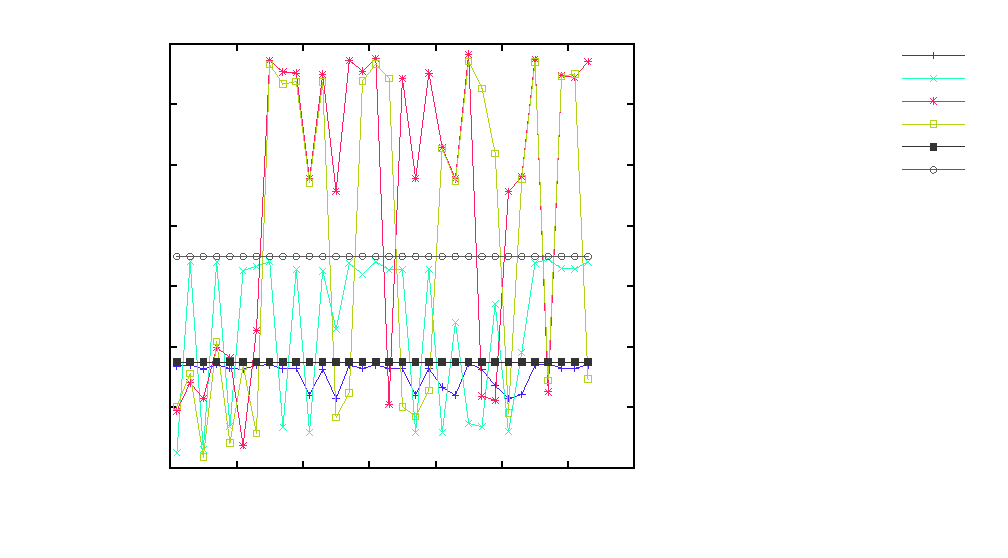
\includegraphics{graph1}}%
    \gplfronttext
  \end{picture}%
\endgroup

    %\caption{Speed of height calculations performed on a subdivided surface} 
    \label{runtimes}
\end{figure}

\begin{table}  [ht]
    \centering
        \begin{tabular}{lllll}
%        \hline
          threads & course, dynamic & course, static & fine, dynamic & fine, static \\ \hline
          1       & 63.876          & 63.143         & 24.969        & 50.671       \\ 
          2       & 99.098          & 100.351        & 10.835        & 23.741       \\ 
          4       & 160.353         & 152.559        & 10.849        & 17.366       \\ 
          6       & 202.808         & 184.358        & 8.774         & 1.173        \\ 
          8       & 15.103          & 53.048         & 0.744         & 12.640       \\ 
           10      & 89.957          & 75.693         & 1.460         & 1.480        \\ 
           12      & 83.028          &  66.268        & 1.246         & 1.302        \\ 
           14      & 81.970          & 53.221         & 1.119         & 1.127        \\ 
           16      & 73.886          & 48.399         & 0.999         & 1.021        \\
%        \hline
            \end{tabular}
    \end{table}

%\begin{figure} [ht]
    %\centering
    %\input{plot_difference.tex}
    %\caption{A run with with percent speedup calculated. simd mflops/non-simd mflops} 
    %\label{runtimes}
%\end{figure}



    \end{document}
